\documentclass[12pt]{article}

\usepackage[english]{babel}
\usepackage[utf8x]{inputenc}
\usepackage{amsmath}
\usepackage{enumitem}
\usepackage{graphicx}
\usepackage{ulem}
\usepackage{caption}
\usepackage{placeins}
\usepackage[usenames,dvipsnames]{color}
\usepackage[colorinlistoftodos]{todonotes}
\usepackage{listings}
\usepackage{fixltx2e}
\usepackage{scrpage2}
\usepackage{lastpage}
\clearscrheadfoot
\pagestyle{scrheadings}
\usepackage{glossaries}
\usepackage[
top    = 2.75cm,
bottom = 2.00cm,
left   = 2.50cm,
right  = 2.00cm]{geometry}
\setcounter{secnumdepth}{4}


\makeglossaries

\newglossaryentry{db} {name=DB, description={Database}}
\newglossaryentry{er} {name=ER, description={Entity Relationship}}


\begin{document}
\begin{titlepage}
\begin{center}
% Oberer Teil der Titelseite:

\includegraphics[width=0.5\textwidth]{images/logo}\\[1cm]    

\textsc{\LARGE Technologisches Gewerbe Museum}\\[1.5cm]

% Title
\rule{12cm}{1mm}
{ \huge \bfseries  \\\large VSDB\\ \huge Synchronisation von Heretogenen DBs \\[0.4cm] }

\rule{12cm}{1mm}

% Author and supervisor
\noindent 
\vspace{5cm}

\begin{center}
\large
Author: 
Schrack \textsc{Nikolas} \&
Siegel \textsc{Hannah}
\end{center}

\vfill

% Bottom of the page
{\large \today}

\end{center}
\end{titlepage}

\tableofcontents


%HEADER AND FOOTER
\pagenumbering{arabic}
\automark{section}
\ifoot{© Schrack, Siegel}
\ofoot{\pagemark ~of \pageref{LastPage}}

\newpage
\section{Arbeitszeit}
\subsection{Geschaetzte Arbeitszeit}
\begin{table}[h]

\begin{tabular}{|p{0.4\textwidth}|p{0.2\textwidth}|p{0.2\textwidth}|}
\hline
\textbf{Task}    & \textbf{Person}                                               & \textbf{Time in hours                              } \\ \hline \hline
Einlesen und Vergleich von gaengigen Middleware-produkten & \begin{tabular}[c]{c}Schrack \\ Siegel \end{tabular} & \begin{tabular}[c]{c}1\\ 1\end{tabular}    \\ \hline 
Implementierung der Middleware & \begin{tabular}[c]{c}Schrack \\ Siegel \end{tabular} & \begin{tabular}[c]{c}5\\ 5\end{tabular}    \\ \hline
Erstellen der Tables, inserts & \begin{tabular}[c]{c}Schrack \\ Siegel \end{tabular} & \begin{tabular}[c]{c}1\\ 1\end{tabular}    \\ \hline
Test mit mehr als einer Tabelle  & \begin{tabular}[c]{c}Schrack \\ Siegel \end{tabular} & \begin{tabular}[c]{c}2\\ 2\end{tabular}    \\ \hline
Dokumenation der Funktionsweise, Problematiken und Problemfälle, sowie allgemeine Dokumentation
  & \begin{tabular}[c]{c}Schrack \\ Siegel \end{tabular} & \begin{tabular}[c]{c}1\\ 1\end{tabular}    \\ \hline
  Testfaelle  & \begin{tabular}[c]{c}Schrack \\ Siegel \end{tabular} & \begin{tabular}[c]{c}2\\ 2\end{tabular}    \\ \hline
 \hline
Total & \begin{tabular}[c]{c}Schrack \\ Siegel \end{tabular} & \begin{tabular}[c]{c}12\\12\end{tabular}   \\ \hline 
\textbf{Gesammt Team} & & \textbf{24 hours}  \\ \hline 
\end{tabular}
\caption{Estimated working time}
\label{tabel:tab1}
\end{table}
\newpage
\subsection{Tatsaechliche Arbeitszeit}
\begin{table}[h]

\begin{tabular}{|p{0.4\textwidth}|p{0.2\textwidth}|p{0.2\textwidth}|}
\hline
\textbf{Task}    & \textbf{Person}                                               & \textbf{Time in hours                              } \\ \hline \hline
Einlesen und Vergleich von gaengigen Middleware-produkten & \begin{tabular}[c]{c}Schrack \\ Siegel \end{tabular} & \begin{tabular}[c]{c}0.5\\ 0.5\end{tabular}    \\ \hline 
Implementierung der Middleware & \begin{tabular}[c]{c}Schrack \\ Siegel \end{tabular} & \begin{tabular}[c]{c}0\\ 0\end{tabular}    \\ \hline
Implementierung der Middleware & \begin{tabular}[c]{c}Schrack \\ Siegel \end{tabular} & \begin{tabular}[c]{c}0\\ 0\end{tabular}    \\ \hline
Implementierung der Middleware & \begin{tabular}[c]{c}Schrack \\ Siegel \end{tabular} & \begin{tabular}[c]{c}0\\ 0\end{tabular}    \\ \hline

Erstellen der Tables, inserts & \begin{tabular}[c]{c}Schrack \\ Siegel \end{tabular} & \begin{tabular}[c]{c}2 \\ 2\end{tabular}    \\ \hline
Test mit mehr als einer Tabelle  & \begin{tabular}[c]{c}Schrack \\ Siegel \end{tabular} & \begin{tabular}[c]{c}2\\ 2\end{tabular}    \\ \hline
Dokumenation der Funktionsweise, Problematiken und Problemfälle, sowie allgemeine Dokumentation
  & \begin{tabular}[c]{c}Schrack \\ Siegel \end{tabular} & \begin{tabular}[c]{c}1\\ 1\end{tabular}    \\ \hline
  Testfaelle  & \begin{tabular}[c]{c}Schrack \\ Siegel \end{tabular} & \begin{tabular}[c]{c}2\\ 2\end{tabular}    \\ \hline
 \hline
Total & \begin{tabular}[c]{c}Schrack \\ Siegel \end{tabular} & \begin{tabular}[c]{c}12\\12\end{tabular}   \\ \hline 
\textbf{Gesammt Team} & & \textbf{24 hours}  \\ \hline 
\end{tabular}
\caption{Estimated working time}
\label{tabel:tab1}
\end{table}

\section{Arbeitsdurchfuehrung}
\subsection{Entwerfen der Datenbank}
Wir haben uns entschieden, eine ganz normale Firma abzubilden, wie sehr oft verwendet bei solchen test beispielen. \\
Es soll einen Mitarbeiter/Person geben, welcher einen namen hat, welcher sich unterscheiden soll. Weiters soll dieser Mitarbeiter bei einer Abteilung arbeiten (um eine 1:n Beziehung abzubilden), und als Teilnehmer bei einer Veranstaltung teilnehmen (um eine n:m Beziehung abzubilden). \\
Des weiteren werden wir darauf achten, moeglichst unterschiedliche und komplexe datentypen zu verwenden.
Wir haben unter \cite{crossmapping} gelesen, dass zum Beispiel boolean unter mysql und pgsql unterschiedlich ist.
\newpage
\subsubsection{PgSQL}
\begin{figure}[here!]
\centering
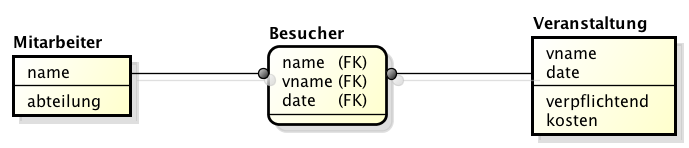
\includegraphics[width=0.8\textwidth]{images/ERD_psql.png}
\caption{\gls{er} fuer pgSQL}
\end{figure}
\FloatBarrier
\subsubsection{Mysql}
\begin{figure}[here!]
\centering
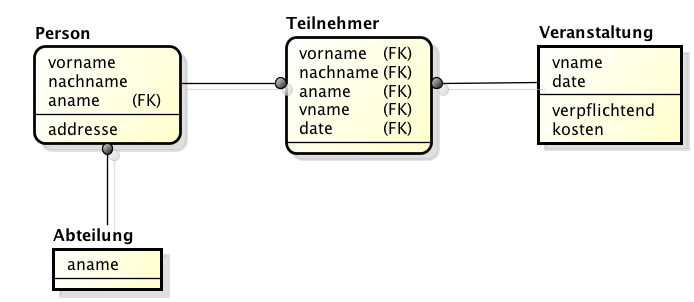
\includegraphics[width=0.8\textwidth]{images/ERD_mysql.png}
\caption{\gls{er} fuer mysql}
\end{figure}
\FloatBarrier

\newpage
\listoffigures
\printglossaries
\begin{thebibliography}{56}


 \bibitem{crossmapping} 
  \textbf{Roland Bouman}, Dec 21 '09 um 21:36\\
  \textit{http://stackoverflow.com/questions/1942586/comparison-of-database-column-types-in-mysql-postgresql-and-sqlite-cross-map}
  \newline zuletzt abgerufen: 2014-10-24 09:00
\end{thebibliography}
\newpage
\end{document}
